I test sono stati condotti variando il numero di piani e le dimensioni delle immagini.
Prima dell'esecuzione dei test, sono stati generati tutti i piani e i cerchi in modo da garantire un confronto accurato
tra i diversi metodi di parallelizzazione.
Le dimensioni delle immagini utilizzate sono 256x256, 512x512 e 1024x1024.

Il numero di piani varia da 1000 a 10000, con un incremento di 1000 piani per i test con risoluzioni 256x256 e 512x512.
Per il test con risoluzione 1024x1024, il numero di piani varia da 100 a 1000, con un incremento di 100 piani.

Le versioni delle librerie utilizzate sono OpenCV 4.6.0 e CUDA 11.8.

\subsection{Generazione}\label{subsec:generazione}
\begin{table}[H]
    \centering
    \begin{tabular}{c|c|c|c|c|c|c|}
        & \multicolumn{2}{|c|}{$N = 100$} & \multicolumn{2}{|c|}{$N = 1000$} & \multicolumn{2}{|c|}{$N = 10000$} \\
        & $n=50$ & $n=500$ & $n=50$ & $n=500$ & $n=50$ & $n=500$ \\
        \hline
        Sequential & TODO & TODO & TODO & TODO & TODO & TODO \\
        Parallel & TODO & TODO & TODO & \textbf{TODO} & TODO & \textbf{TODO} \\
    \end{tabular}
    \caption{\label{tab:gen}Tempi impiegati per la generazione dei cerchi e dei piani}
\end{table}

\subsection{256x256}\label{subsec:256x256}
\begin{figure}[H]
    \centering
    \begin{minipage}{0.49\textwidth}
        \centering
        \includegraphics[width=\textwidth]{plots/256/omp_times}
        \caption{Tempi di OMP}\label{fig:times-256-omp}
    \end{minipage}
    \begin{minipage}{0.49\textwidth}
        \centering
        \includegraphics[width=\textwidth]{plots/256/omp_speedup}
        \caption{Speedup di OMP}\label{fig:speedup-256-omp}
    \end{minipage}
\end{figure}

\begin{figure}[H]
    \centering
    \begin{minipage}{0.49\textwidth}
        \centering
        \includegraphics[width=\textwidth]{plots/256/cuda_times}
        \caption{Tempi di CUDA}\label{fig:times-256-cuda}
    \end{minipage}
    \begin{minipage}{0.49\textwidth}
        \centering
        \includegraphics[width=\textwidth]{plots/256/cuda_speedup}
        \caption{Speedup di CUDA}\label{fig:speedup-256-cuda}
    \end{minipage}
\end{figure}

\begin{figure}[H]
    \centering
    \begin{minipage}{0.49\textwidth}
        \centering
        \includegraphics[width=\textwidth]{plots/256/results_times}
        \caption{Confronto dei tempi}\label{fig:tempi-256}
    \end{minipage}
    \begin{minipage}{0.49\textwidth}
        \centering
        \includegraphics[width=\textwidth]{plots/256/results_speedup}
        \caption{Confronto fra speedups}\label{fig:speedups-256}
    \end{minipage}
\end{figure}

\subsection{512x512}\label{subsec:512x512}
\begin{figure}[H]
    \centering
    \begin{minipage}{0.49\textwidth}
        \centering
        \includegraphics[width=\textwidth]{plots/512/omp_times}
        \caption{Tempi di OMP}\label{fig:times-512-omp}
    \end{minipage}
    \begin{minipage}{0.49\textwidth}
        \centering
        \includegraphics[width=\textwidth]{plots/512/omp_speedup}
        \caption{Speedup di OMP}\label{fig:speedup-512-omp}
    \end{minipage}
\end{figure}

\begin{figure}[H]
    \centering
    \begin{minipage}{0.49\textwidth}
        \centering
        \includegraphics[width=\textwidth]{plots/512/cuda_times}
        \caption{Tempi di CUDA}\label{fig:times-512-cuda}
    \end{minipage}
    \begin{minipage}{0.49\textwidth}
        \centering
        \includegraphics[width=\textwidth]{plots/512/cuda_speedup}
        \caption{Speedup di CUDA}\label{fig:speedup-512-cuda}
    \end{minipage}
\end{figure}

\begin{figure}[H]
    \centering
    \begin{minipage}{0.49\textwidth}
        \centering
        \includegraphics[width=\textwidth]{plots/512/results_times}
        \caption{Confronto dei tempi}\label{fig:tempi-512}
    \end{minipage}
    \begin{minipage}{0.49\textwidth}
        \centering
        \includegraphics[width=\textwidth]{plots/512/results_speedup}
        \caption{Confronto fra speedups}\label{fig:speedups-512}
    \end{minipage}
\end{figure}

\subsection{1024x1024}\label{subsec:1024x1024}
\begin{figure}[H]
    \centering
    \begin{minipage}{0.49\textwidth}
        \centering
        \includegraphics[width=\textwidth]{plots/1024/omp_times}
        \caption{Tempi di OMP}\label{fig:times-1024-omp}
    \end{minipage}
    \begin{minipage}{0.49\textwidth}
        \centering
        \includegraphics[width=\textwidth]{plots/1024/omp_speedup}
        \caption{Speedup di OMP}\label{fig:speedup-1024-omp}
    \end{minipage}
\end{figure}

\begin{figure}[H]
    \centering
    \begin{minipage}{0.49\textwidth}
        \centering
        \includegraphics[width=\textwidth]{plots/1024/cuda_times}
        \caption{Tempi di CUDA}\label{fig:times-1024-cuda}
    \end{minipage}
    \begin{minipage}{0.49\textwidth}
        \centering
        \includegraphics[width=\textwidth]{plots/1024/cuda_speedup}
        \caption{Speedup di CUDA}\label{fig:speedup-1024-cuda}
    \end{minipage}
\end{figure}

\begin{figure}[H]
    \centering
    \begin{minipage}{0.49\textwidth}
        \centering
        \includegraphics[width=\textwidth]{plots/1024/results_times}
        \caption{Confronto dei tempi}\label{fig:tempi-1024}
    \end{minipage}
    \begin{minipage}{0.49\textwidth}
        \centering
        \includegraphics[width=\textwidth]{plots/1024/results_speedup}
        \caption{Confronto fra speedups}\label{fig:speedups-1024}
    \end{minipage}
\end{figure}